\section{Implementation}
\label{sec:impl}

In this section, we describe how \lang programs can be evaluated. First, we
detail a variant of semi-naive evaluation that supports lattices. We validate
that our implementation of semi-naive evaluation results in significant
performance gains and is competitive with a traditional set-oriented version of
semi-naive evaluation. We also detail the engineering effort required to extend
Bud to support \lang. % XXX: last sentence is weak

\subsection{Evaluation strategy}
\label{sec:lattice-eval-strat}
\nrc{TODO: describe how we generalize semi-naive to \lang, justify why it is
  correct.}

\emph{Naive} evaluation is a simple but inefficient approach to evaluating
recursive Datalog programs. Evaluation proceeds in ``rounds.'' In each round, all
the rules in the program are evaluated over the entire database (including all
derivations made in previous rounds). This process stops when a round makes no
new derivations. Naive evaluation is inefficient because it makes many redundant
derivations: once a fact has been derived in round $i$, it is rederived in every
subsequent round.

\emph{Semi-naive} evaluation improves upon naive evaluation by making fewer
redundant derivations~\cite{Balbin1987}.

\subsection{Performance validation}
\label{sec:lattice-perf}

\begin{figure}[t]
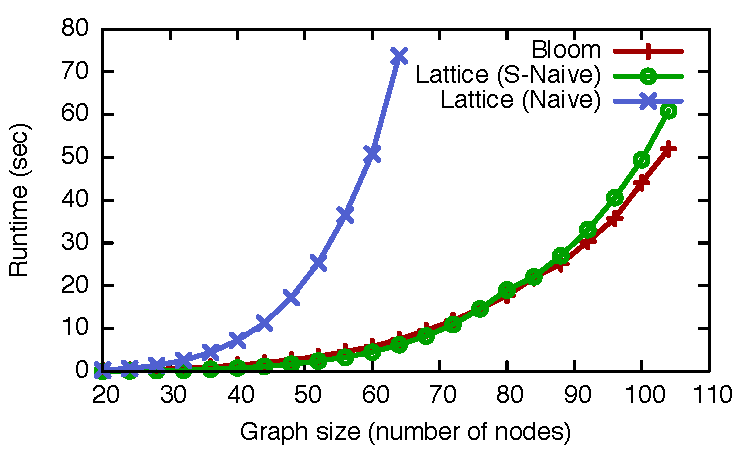
\includegraphics[width=\linewidth]{fig/sn_perf}
\caption{Performance comparison of three different methods for computing the
  transitive closure of a graph.}
\label{fig:tc-perf-graph}
\end{figure}

To validate the effectiveness of semi-naive evaluation for \lang programs, we
wrote two versions of a program to compute the transitive closure of a directed
acyclic graph. One version was written in Bloom and used traditional
set-oriented collections. The other version was written in \lang and used
morphisms over the \texttt{lset} lattice. For the \lang version, we ran the
program both with and without semi-naive evaluation enabled. As input, we used
synthetic graphs of various sizes---in a graph with $n$ nodes, each node had
$O(\log_2 n)$ outgoing edges. We ran the experiment on a late 2010 MacBook Air
with a 2.13 Ghz Intel Core 2 Duo processor and 4GB of RAM, running Mac OS X
10.7.3 and Ruby 1.8.7-p352. We ran each program variant five times on each graph
and report the mean elapsed wall-clock time.

Figure~\ref{fig:tc-perf-graph} shows how the runtime of each program varied with
the size of the graph. Note that we only report results for the naive \lang
strategy on small input sizes because this variant ran very slowly as the graph
size increased. The poor performance of naive evaluation is not surprising:
after deriving all paths of length $n$, naive evaluation will then rederive all
those paths at every subsequent ``step'' of the fixpoint computation. In
contrast, after computing length $n$ paths, a semi-naive strategy will only
generate length $n+1$ paths in the next step. Bloom and semi-naive \lang achieve
similar results. We instrumented Bud to count the number of derivations made by
the Bloom and semi-naive lattice variants---as expected, both programs made about
the same number of derivations. These results suggest that our implementation of
semi-naive evaluation for \lang is effective and performs comparably with a
traditional Datalog system.

For large inputs, Bloom begins to outperform the semi-naive lattice variant. We
suspect this is because our current implementation of lattices requires more
data copies. Lattices are immutable, so the \texttt{lset} merge function
allocates a new set to hold the result of the merge. In contrast, Bloom
collections are modified in-place. We plan to improve our lattice implementation
to avoid copying lattice values when the interpreter can prove that in-place
updates are safe.

\subsection{Modifying Bud}
We were able to extend Bud to support \lang with relatively minor changes. Bud
initially had about 7200 lines of Ruby source code (LOC). The core lattice
features (the \texttt{Bud::Lattice} base class and the mapping from identifiers
to lattice elements) required about 300 LOC. Modifying Bud's fixpoint logic to
include lattices required only 10 LOC, while the program rewriting required to
enable semi-naive evaluation required 100 LOC. Modifying Bud's collection
classes to support merging of embedded lattice values required modifying about
125 LOC. The builtin lattice classes constituted an additional 300 LOC. In
total, adding support for \lang required less than 900 lines of added or
modified code, and took about two man-months of engineering time.%  This
% experience suggests that support for lattices can be added to an existing
% Datalog engine in a relatively straightforward manner.
